% !TEX program = xelatex

\documentclass[14pt]{extarticle}
\usepackage[utf8x]{inputenc}
\usepackage[english,russian]{babel}
\usepackage{indentfirst}
\usepackage{graphicx}
\usepackage{amsmath}
\usepackage{amsfonts}
\usepackage{longtable}


% Set line spacing
\usepackage{leading}
\leading{18pt}


% Set font
\usepackage{fontspec}
\setmainfont{Times New Roman}


% Set paper size and margins
\usepackage{geometry}
\geometry{
	a4paper,
	top=2cm,
	bottom=2cm,
	left=3cm,
	right=1cm,
	bindingoffset=0cm,
}


% Package for code blocks
\usepackage{verbatim}
\makeatletter
\newcommand{\verbatimfont}[1]{\renewcommand{\verbatim@font}{\ttfamily#1}}


\author{Даниил Крачковский}
\title{Дипломная работа}


% Change table of contents title
% \addto\captionsrussian{\renewcommand{\contentsname}{Оглавление}}


\begin{document}

	\begin{titlepage}

  \begin{center}
    \textbf{БЕЛОРУССКИЙ ГОСУДАРСТВЕННЫЙ УНИВЕРСИТЕТ} \\
    \textbf{Факультет прикладной математики и информатики} \\
    \textbf{Кафедра вычислительной математики}
  \end{center}

  \vfill

  \begin{center}
    Аннотация к дипломной работе
  \end{center}

  % \vspace{1cm}

  \begin{center}
    \textbf{Вычислительные алгоритмы} \\
    \textbf{положительной матричной факторизации}
  \end{center}

  \vspace{1cm}

  \begin{center}
    Крачковский Даниил Янович
  \end{center}

  \vspace{1.5cm}

  \begin{center}
    Научный руководитель -
    кандидат физико-математических наук, доцент \\ Фалейчик Б. В.
  \end{center}

  \vfill

  \begin{center}
    \textbf{
      Минск, \the\year
    }
  \end{center}

\end{titlepage}


	\tableofcontents{}

	% Введение:
% - О задаче НМФ
% - в чем трудности
% - где применяется
% - постановка задачи
% - что сделано в работе
% - кратко о полученных результатах

% \newpage

\chapter*{ВВЕДЕНИЕ}
\addcontentsline{toc}{chapter}{Введение}

На сегодняшний день объемы информации растут в геометрической прогрессии.
Ярким примером  скопления обширного количества данных является социальная сеть Instagram переступившая порог в 1 млрд пользователей.
Для того чтобы быстрее реагировать на изменения рынка, получить конкурентные преимущества,
повысить эффективность сервиса нужно получить, обработать и проанализировать огромное количество данных.
Обработка таких больших объемов данных создаёт новые проблемы в отношении представления данных,
упразднения неоднозначности и уменьшения размерности.

Неотрицательная матричная факторизация (НМФ) - это метод уменьшения размерности.
Многие методы уменьшения размерности тесно связаны с приближениями матрицами низкого ранга,
и неотрицательная матричная факторизация является особенной в том,
что искомые матрицы низкого ранга ограничены только неотрицательными элементами.
За последнее десятилетие
неотрицательная матричная факторизация получила огромное внимание и была успешно применена в широком спектре
важных проблем в таких областях, как интеллектуальный анализ текста, компьютерное зрение,
биоинформатика, спектральный анализ данных, разделение слепых источников и многих других.

Во многих ситуациях данные, наблюдаемые из сложных процессов и взаимодействий
представляют собой совокупный результат нескольких взаимосвязанных переменных, действующих вместе.
Когда эти переменные определены с некоторыми неточностями, фактическая информация, содержащаяся в исходных данных,
может перекрываться и быть неоднозначной.
В данном случае модель с упрощённой системой может обеспечить точность около уровня точности исходной системы.
Одна общая идея в различных подходах к устранению шума, уменьшению размерности модели,
восстановлению непротиворечивости и т.д. заключается в замене исходных данных данными меньшей размерности,
полученными с помощью аппроксимации некоторым подпространством.
Эта идея получила название аппроксимации низкого ранга.
Использование аппроксимации низкого ранга выходит на передний план в широком спектре важных задач.
Факторный анализ и метод главных компонент являются двумя из многих классических методов,
используемых для достижения цели сокращения числа переменных и выявления структур среди переменных.

Часто анализируемые данные неотрицательны, что накладывает следующие ограничения на аппроксимирующие данные:
данные более низкого ранга также должны состоять из неотрицательных значений, чтобы избежать противоречий с природой исходных данных.
Классические инструменты не могут гарантировать сохранение неотрицательности.
Таким образом, естественным выбором становится поиск неотрицательных множителей пониженного ранга для аппроксимации данной неотрицательной матрицы данных.

Цель настоящей работы состоит в исследовании эффективности алгоритмов неотрицательной матричной факторизации и их применение к задаче интеллектуального анализа текста.

В ходе работы было программно реализовано 4 метода решения задачи НМФ
(метод мультипликативного обновления и 3 различных модификации метода попеременных наименьших квадратов), проведено их экспериментальное сравнение.
Реализованные алгоритмы были применены к задаче выделения ключевых слов и предложений в текстах.

	% НМФ
% - четко о постановке задачи,
% - описание реализованных методов (отдельный пункт для каждого метода + код),
% - о сходимости (см. статью))

\chapter{Неотрицательная матричная факторизация}





\section{Постановка задачи}

Задача неотрицательной матричной факторизации может быть сформулирована следующим образом:
Для матрицы $A \in R^{m \times n}, A \geq 0$ и числа $k \in N, k < \min\{n, m\}$
необходимо найти  такие матрицы $W \in R^{m \times k}, H \in R^{k \times n} : W \geq 0, H \geq 0$ чтобы было верным приближенное равенство:
\begin{equation} \label{eq:problem}
  A \approx W H
\end{equation}

Произведение $WH$ называется неотрицательной факторизацией матрицы $A$. Неравенства $A \geq 0$, $W \geq 0$, $H \geq 0$ означают что все элементы соответствующих матриц неотрицательны.
Качество приближения по формуле \eqref{eq:problem} можно оценить различными способами, такими как норма Фробениуса,
дивергенция Кульбака-Лейблера и некоторыми другими.

Дивергенция Кульбака-Лейблера:
\begin{equation*}
  f(W, H) =
    \sum_{i=1}^m \sum_{j=1}^n
    \left(
      A_{i,j} \
      ln\left(
        \frac{A_{i,j}}{(WH)_{i,j}}
      \right)
      - A_{i,j}
      + (WH)_{i,j}
    \right)
\end{equation*}

Норма Фробениуса:
\begin{equation*}
  f(W, H) = || A - WH ||^2_F
\end{equation*}

Ниже будет использован несколько модифицированный вариант нормы Фробениуса,
который называется относительной нормой Фробениуса:
\begin{equation} \label{eq:frob_norm}
  f(W, H) = \dfrac{||A - WH||_F}{|| A ||_F}
\end{equation}

В идеальном случае, когда $f(W,H)=0$ матрица $A$ равна произведению $WH$.
На практике это далеко не всегда так, и почти всегда произведение $WH$ является приближенным разложением ранга не более $k$.

\newpage

Учитывая все вышесказанное задачу неотрицательной матричной факторизации можно сформулировать следующим образом:

\subsubsection{Задача неотрицательной матричной факторизации}

Для матрицы $A \in R^{m \times n}, A \geq 0$ и числа $k \in N, k < \min\{n, m\}$
необходимо найти матрицы $W \in R^{m \times k}, H \in R^{k \times n} : W \geq 0, H \geq 0$ минимизируя функционал:
\begin{equation} \label{eq:min_problem}
  \min_{W \geq 0, \ H \geq 0} \dfrac{||A - WH||_F}{|| A ||_F}
\end{equation}

Задача \eqref{eq:min_problem} является невыпуклой задачей оптимизации относительно переменных $W$ и $H$,
и нахождение ее глобального минимума является NP-сложной задачей \cite{vavaris}.
Поэтому ожидается, что хороший алгоритм будет вычислять некоторый удовлетворительный локальный минимум задачи \eqref{eq:min_problem}.

Правильный выбор значения $k$ является критически важным для получения удовлетворительного результата,
но также выбор $k$ очень часто зависит от природы решаемой задачи и поставленного вопроса.
В большинстве случаев, $k$ обычно выбирают таким образом, чтобы $k \ll \min\{m, n\}$,
и в этом случае произведение $WH$ можно рассматривать как сжатую форму данных матрицы $A$.

Ключевой характеристикой неотрицательной матричной факторизации является возможность
использования численных методов для минимизации \eqref{eq:min_problem}
для извлечения некоторых базовых признаков в качестве базисных векторов матрицы $W​$,
которые затем могут быть использованы для поиска и классификации.
Ограничивая матрицы $W​$ и $H​$ только неотрицательными элементами
неотрицательная матричная факторизация позволяет представлять исходные данные из \textit{не вычитающих комбинаций}.
Элементы таких комбинаций могут быть частями лиц в изображениях, темами или кластерами в текстовых данных
или некоторыми другими характеристиками многомерных данных.

Одной их важных проблем, влияющих на численную минимизацию \eqref{eq:min_problem},
является существование локальных минимумов
из-за невыпуклости \eqref{eq:min_problem} как по $W$, так и по $H$.
Не менее важной проблемой является отсутствие единственного решения,
которое можно легко увидеть рассматривая произведение $WDD^{− 1}H$ для любой неотрицательной обратимой матрицы $D$.

Несмотря на многие недостатки неотрицательная матричная факторизация весьма привлекательна для приложений интеллектуального анализа данных,
поскольку на практике даже локальные минимумы могут обеспечивать желаемые свойства, такие как сжатие данных и извлечение базовых признаков.





\newpage





\section{Методы решения задачи}

Существует множество различных способов решения задачи неотрицательной матричной факторизации.
Самыми популярными и наиболее исследованным являются: метод главных компонент, усеченное сингулярное разложение и методы неотрицательной матричной факторизации.
Стоит отметить что все вышеперечисленные методы решают задачу неотрицательной матричной факторизации,
однако название \textit{"метод неотрицательной матричной факторизации"} обычно применимо только к методам решающим задачу в формулировке \eqref{eq:min_problem}.
Ниже будут рассмотрены некоторые методы численного решения задачи неотрицательной матричной факторизации.

\subsubsection{Численные методы решения задачи}
Численные методы решения задачи неотрицательной матричной факторизации
могут быть поделены на следующие основные категории:
\begin{enumerate}
	\item Методы мультипликативного обновления
	\item Методы попеременных наименьших квадратов
	\item Методы градиентного спуска
\end{enumerate}

К методам мультипликативного обновления принадлежит классический метод мультипликативного обновления,
разработанный Lee и Seung \cite{lee_seung},
а также множество основанных на нём методов улучшающих его сходимость.

К методам попеременных наименьших квадратов относится множество методов,
использующих тот факт, что задача разрешима отдельно по каждой переменной.

К методам градиентного спуска относятся такие методы, как метод проецированного градиентного спуска \cite{lin} и другие.

В ходе работы были исследованы 2 категории методов: методы мультипликативного обновления и методы попеременных наименьших квадратов.
Далее будут подробнее рассмотрены самые распространенные методы из этих категорий.



\newpage



\subsection{Метод мультипликативного обновления}

Алгоритм был разработан Daniel D. Lee и H. Sebastian Seung в 2001 году.
Lee и Seung использовали градиент и свойства непрерывного спуска (точнее, непрерывного невозрастания),
чтобы утверждать, что данный алгоритм сходится к локальному минимуму.
Фактически, доказательство показывает свойство непрерывного спуска (невозрастания),
которое не исключает достижения только локального минимума.

\begin{algorithm}
  \BlankLine
  \BlankLine

  \Input{Неотрицательная матрица $A$}
  \Output{Неотрицательные матрицы $W$ и $H$}

  \BlankLine

  Инициализировать $W$ и $H$ как случайные плотные матрицы\;

  \While{не достигнут критерий останова} {
    Обновить $H$ значением $H * W^T A / (W^T W H + \epsilon)$\;
    Обновить $W$ значением $W * A H^T / (W H H^T + \epsilon)$\;
  }

  \BlankLine

  \caption{Алгоритм мультипликативного обновления}
\end{algorithm}

Добавление $\epsilon$ в каждом правиле обновления необходимо чтобы избежать деления на ноль.
Обозначение $*$ подразумевает покомпонентное умножение матриц.

Если исходные матрицы $W$ и $H$ неотрицательны, то эти матрицы остаются неотрицательными на протяжении всех итераций.
Это утверждение легко подтверждается опираясь на мультипликативную форму правил обновления.

Благодаря своему статусу первых известных алгоритмов неотрицательной матричной факторизации
алгоритмы мультипликативного обновления стали основой,
с которой сравниваются более новые алгоритмы.
Неоднократно было показано \cite{langville}, что данные алгоритмы медленно сходятся.
Они требуют намного больше итераций, чем альтернативы, такие как алгоритмы градиентного спуска и попеременных наименьших квадратов, и работа на одну итерацию высока.
Каждая итерация требует шести $O(n^3)$ матричных умножений полностью плотных матриц и шести $O(n^2)$ покомпонентных умножений матриц.
Тем не менее, хорошие реализации могут улучшить ситуацию.
Например, в правиле обновления для $W$, для которого требуется произведение $WHH^T$, сначала необходимо вычислить малое $k \times k$ произведение $HH^T$.

\newpage

Ниже приведена реализация данного алгоритма на языке программирования \textit{Python 3}.
\\

\lstinputlisting
  [caption=Реализация алгоритма MU на python3]
  {../src/methods/multiplicative_update_rule.py}



\newpage



\subsection{Метод попеременных наименьших квадратов}

В этом методе за шагом наименьших квадратов следует другой шаг наименьших квадратов поочередно.
Впервые методы попеременных наименьших квадратов были использованы в работе Paatero \cite{paatero}.

Метод использует тот факт, что задача минимизации выражения \eqref{eq:min_problem} не является выпуклой как в $W$,
так и в $H$ одновременно, но является выпуклой в $W$ или $H$ по отдельности.
Таким образом, для одной матрицы другая матрица может быть найдена решением простой задачи наименьших квадратов.

\begin{algorithm}
  \BlankLine
  \BlankLine

  \Input{Неотрицательная матрица $A$}
  \Output{Неотрицательные матрицы $W$ и $H$}

  \BlankLine

  Инициализировать  $W$ и $H$ как случайные плотные матрицы\;

  \While{не достигнут критерий останова} {
    Найти $H$ решая задачу $\displaystyle\min_H||WH - A||$\; \label{alg:line:lstsq_1}
    Спроецировать $H$ на неотрицательную область\;
    Найти $W$ решая задачу $\displaystyle\min_{W^T}||H^TW^T - A^T||$\; \label{alg:line:lstsq_2}
    Спроецировать $W$ на неотрицательную область\;
  }

  \BlankLine

  \caption{Алгоритм попеременных наименьших квадратов}
\end{algorithm}

В приведенном выше алгоритме используется простейший метод сохранения неотрицательности:
проецирование матрицы на неотрицательную область.

На самом деле проецирование просто устанавливает все отрицательные элементы, полученные в результате
вычисления решения, в $0$.

Эта простая техника также имеет несколько дополнительные преимуществ:
она способствует разреженности матрицы, а кроме того добавляет гибкости итерациям,
которая недоступна в других алгоритмах, особенно в алгоритмах мультипликативного обновления.
Одним из недостатков алгоритмов мультипликативного обновления является то,
что если элемент в $W$ или $H$ становится равным $0$,
то он будет оставаться равным $0$ на протяжении всех итераций.
Эта блокировка нулевых элементов является большим ограничением алгоритма,
что означает как только алгоритм начинает двигаться вниз по пути к фиксированной точке,
даже если это \say{плохая} фиксированная точка, алгоритм продолжит двигаться в направлении к этой точке.
Алгоритмы попеременных наименьших квадратов являются более гибкими,
позволяя итеративному процессу сойти с \say{плохого} пути.




\newpage




Существует множество различных реализаций метода наименьших квадратов.
Каждая реализация основывается на различном методе решения задачи наименьших квадратов.

Далее рассмотрены самые популярные и эффективные реализации метода попеременных наименьших квадратов.

\subsubsection{Метод нормальных уравнений}

Данный алгоритм является базовым из семейства алгоритмов попеременных наименьших квадратов.
Задач наименьших квадратов решается следующим способом.
Необходимо находить значения $W$ и $H$ на каждой итерации и приведённых ниже уравнений.
\begin{equation}
  W^T W H = W^T A
\end{equation}
\begin{equation}
  H H^T W^T = H A^T
\end{equation}


На практике алгоритм очень чувствителен к накапливанию вычислительной погрешности,
а также, хоть поддерживает работу с разреженными матрицами, имеет проблемы при работе с вырожденными матрицами.
Так как разреженные матрицы обычно имеют не полный, весьма маленький ранг,
велика вероятность того, что одна из матриц $W^TW$, $HH^T$ также будет не полного ранга.
Ситуации такого рода ведут к невозможности продолжения итерационного процесса.

\newpage

Ниже приведена реализация данного алгоритма на языке программирования \textit{Python 3}.
\\

\lstinputlisting
  [caption=Реализация алгоритма ALS\_NORM на python3, firstline=32, lastline=53]
  {../src/methods/alternating_least_squares.py}

\newpage

\subsubsection{Метод LSQR}

Следующий метод полностью основан на классическом методе попеременных наименьших квадратов.
В метод внесены корректировки, устраняющие недостатки предшественника, такие как проблемы
с матрицами неполного ранга и накопление вычислительной погрешности.
Для решения задачи наименьших квадратов используется алгоритм LSQR \cite{lsqr}.
\begin{equation}
  \min_H||W^TWH - W^TA||_2
\end{equation}
\begin{equation}
  \min_{W^T}||HH^TW^T - HA^T||_2
\end{equation}

Вместо решения системы линейных алгебраических уравнений на каждом шаге,
метод решает задачу минимизации $\displaystyle\min_X||AX - B||_2$, где $A$, $B$ и $X$ - матрицы.
Это позволяет избежать вышеперечисленных проблем,
однако повышает вычислительную сложность алгоритма.
Также в методе присутствует описанный выше шаг проецирования матрицы
на неотрицательную область.
Стоит отметить, что данный шаг \say{портит} решение, но он необходим,
чтобы обеспечить неотрицательность искомого разложения.

\newpage

Ниже приведена реализация данного алгоритма на языке программирования \textit{Python 3}.
\\

\lstinputlisting
  [caption=Реализация алгоритма ALS\_LSQR на python3, firstline=64, lastline=73]
  {../src/methods/alternating_least_squares.py}



\newpage


\subsubsection{Метод попеременных неотрицательных наименьших квадратов}

Данный метод вносит свои корректировки в метод попеременных наименьших квадратов,
улучшающие его характеристики.
\begin{equation}
  \min_{H \geq 0}||W^TWH - W^TA||_2
\end{equation}
\begin{equation}
  \min_{W^T \geq 0}||HH^TW^T - HA^T||_2
\end{equation}

Вместо решения системы линейных алгебраических уравнений на каждом шаге,
данный метод решает задачу минимизации $\displaystyle\min_{X \geq 0}||AX - B||_2$, где $A$, $B$ и $X$ - матрицы.
Необходимо обратить внимание на то, что на матрицу $X$ накладывается ограничение неотрицательности,
что позволяет избежать применения шага проецирования матрицы неотрицательную область.
На практике это позволяет значительно повысить скорость сходимости,
однако влечёт за собой увеличение вычислительной сложности алгоритма.

\newpage

Ниже приведена реализация данного алгоритма на языке программирования \textit{Python 3}.
\\

\lstinputlisting
  [caption=Реализация алгоритма ALS\_NNLS на python3, firstline=55, lastline=61]
  {../src/methods/alternating_least_squares.py}





\newpage





\section{Алгоритм инициализации матриц $W$ и $H$}

Проблема изложенных алгоритмов неотрицательной матричной факторизации заключается в том,
что сходимость к глобальному минимуму не гарантируется.
Часто случается, что сходимость медленная и достигается неоптимальное приближение.

Эффективная процедура для вычисления хорошего начального приближения может быть основана на сингулярном разложении матрицы $A$ \cite{elden}.

\begin{algorithm}

  \BlankLine
  \BlankLine

  \Input{Неотрицательная матрица $A$}
  \Output{Неотрицательные матрицы $W$ и $H$}

  \BlankLine

  Инициализировать  $W$ и $H$ как случайные плотные матрицы\;
  Factorize $A$ into $U$, $\Sigma$, $V^T$ using SVD\;
  Set $u_1$ as firts column of $U$\;

  \For{$i$ \KwFrom 1 \KwTo $k$} {
    Compute $C$ as $u_i v_i^T$\;
    Project $C$ to nonnegative space\;
    Factorize $C$ into $U^\prime$, $\Sigma^\prime$, $V^{\prime T}$ using SVD\;
    Set $u^\prime_1$ as $i$-th column of $U$\;
  }

  \BlankLine

  \caption{Алгоритм инициализации матриц $W$ и $H$}
\end{algorithm}

Пусть $A = U \Sigma V^T $ является сингулярным разложением для матрицы $A$,
тогда следует взять первый сингулярный вектор $u_1$ в качестве первого столбца в $W$.
Затем необходимо взять матрицу $C = u_2 v_2^T$ и заменить все её отрицательные элементы на ноль.
Так как $C$ теперь является неотрицательной матрицей, то известно, что первый сингулярный вектор этой матрицы также неотрицательный.
Кроме того, предполагая что это достаточно хорошее приближение $u_2$, возможно принять его за второй столбец $W$.
Продолжим процедуру далее, пока вся матрица $W$ не будет заполнена.

На практике метод даёт хороший прирост к сходимости,
однако с ростом размерности исходной матрицы его использование становится
нецелесообразным из-за большой вычислительной сложности.


\newpage

Ниже приведена реализация данного алгоритма на языке программирования \textit{Python 3}.
\\

\begin{lstlisting}[caption=Алгоритм SVD инициализации]
def initialize_svd(A):
  rows, columns = A.shape

  U, _, VT = svd_factorization(A, rank_k)

  W = U[:,:rank_k]
  H = random_matrix(rank_k, columns)

  for j in range(1, rank_k):
    C = reshape(U[:,j], (rows, 1)) @ reshape(VT[j,:], (1, columns))
    C = nonnegative(C)
    u, _, _ = svd_factorization(C, 1)

    W[:,j] = u[:,0]
  return W, H
\end{lstlisting}




\newpage





\section{Сходимость методов решения задачи}

В общем случае, метод неотрицательной матричной факторизации любого класса
должен ввести решение в условие оптимальности \cite{chu},
чтобы определить действительно ли это минимум.
Если решение подходит под условия оптимальности, то это означает, что достигнут как минимум локальный минимум.

На самом деле, задача неотрицательной матричной факторизации некорректно поставлена,
что означает отсутствие единственного глобального минимума.
Необходимо принять во внимание, что минимальное решение, заданное матрицами $W$ и $H$,
также может быть задано бесконечным числом одинаково хороших пар решений,
таких как $WD$ и $D^{-1}H$, для любых неотрицательных $D$ и $D^{−1}$.
Так как масштабирование и перестановка вызывают проблемы уникальности,
некоторые алгоритмы используют нормализацию строк или столбцов на каждой итерации.

Если в конкретном случае необходимо найти \say{достаточно хороший} локальный минимум,
то можно запустить алгоритм неотрицательной матричной факторизации с SVD инициализацией.

\subsubsection{Скорость сходимости}

Доказательство скорости сходимости для этих алгоритмов является открытой нерешённой проблемой.
При определенных условиях возможно говорить о скоростях сходимости выбранных алгоритмов
или сравнивать относительные скорости сходимости между различными алгоритмами.

\subsubsection{Критерий останова}

Для выбора критерия останова необходимо получить оценки качества решения.
Поскольку сингулярное разложение ранга $k$, обозначаемое $U_k \Sigma_k V_k^T$,
обеспечивает нижнюю границу качества, решение должно как минимум удовлетворять следующему неравенству.
\begin{equation*}
  1 - \epsilon \leq \frac{||A - WH||_F}{||A - U_k \Sigma_k V_k^T||_F} \leq 1
\end{equation*}

Где $\epsilon$ - небольшая положительная константа, зависящая от параметров
конкретного алгоритма неотрицательной матричной факторизации.

Естественный критерий сходимости $||A - WH||_F$ требует вычислительных затрат,
которые могут быть немного уменьшены при правильной реализации \cite{berry}.
Следующее альтернативное выражение использует свойства нормы, для уменьшения вычислительных затрат.
\begin{equation} \label{eq:termination}
  ||A - WH||^2_F = \trace (A^T A) - 2 \trace(H^T (W^T A)) + \trace(H^T (W^T W H))
\end{equation}

Данное выражение содержит эффективный порядок матричных произведений и позволяет
единожды произвести вычисления связанные с $\trace(A^T A)$.

Почти все алгоритмы неотрицательной матричной факторизации используют
максимальное количество итераций, как вторичный критерий останова.
Однако очевидно, что фиксированное количество итераций это не математически верный
подход для контроля итерационного процесса и максимальное количество итераций зависит от конкретной прикладной задачи.

Принимая во внимание всё вышесказанное и необходимость работы с разреженными данными,
воспользуемся критерием останова \eqref{eq:termination}.

\newpage

Ниже приведена реализация данного алгоритма на языке программирования \textit{Python 3}.
\\

\lstinputlisting
  [caption=Реализация критерия останова, firstline=18, lastline=34]
  {../src/utils.py}

	% Применение в интеллектуальном анализе данных (ИАД) (общие слова, потом конкретно о тех задачах, на которых будут проводиться тесты)

\newpage
\chapter{Применение в интеллектуальном анализе данных}

Многие методы уменьшения размерности тесно связаны с приближениями матрицами низкого ранга,
и неотрицательная матричная факторизация является особенной в том,
что искомые матрицы низкого ранга ограничены только неотрицательными элементами.
Неотрицательность играет важное значение для данных во многих областях,
в результате чего неотрицательные матрицы низкого ранга приводят к физически естественным интерпретациям искомого приближения.
За последнее десятилетие неотрицательная матричная факторизация получила огромное внимание и была успешно применена к широкому кругу важных проблем в таких областях,
как интеллектуальный анализ текста, компьютерное зрение, биоинформатика, анализ спектральных данных, слепое разделение источников и многим другим.

Ниже будет рассмотрены некоторые алгоритмы интеллектуального анализа текста.





\newpage





\section{Интеллектуальный анализ текста}

Под анализом текста подразумеваются методы извлечения полезной информации из больших и часто неструктурированных коллекций текстов.
Другими словами - поиск информации.
Типичным применением для интеллектуального анализа текста является поиск в базах рефератов научных работ.
Например, в медицинском приложении можно найти все рефераты в базе данных касающиеся определенного синдрома.
Для этого составляют поисковую фразу или запрос с ключевыми словами, которые имеют отношение к синдрому.
Затем используется система поиска для сопоставления запроса с документами в базе данных и представляет пользователю документы,
которые являются релевантными и ранжируются в соответствии с релевантностью.

Очень широко распростанённой областью применения интеллектуального анализа текста
являются поисковые системы в Интернете, где поисковая фраза обычно очень короткая,
и часто имеется так много соответствующих документов, что не представляется возможным предоставить их все пользователю.
В этом случае ранжирование результатов поиска имеет решающее значение для эффективности поисковой системы.

Методы кластеризации документов привлекают все больше и больше внимания
как основной и эффективный инструмент для организации, навигации, поиска и суммирования огромных объемов текстовых документов.
При хорошем методе кластеризации документов компьютеры могут автоматически организовывать наборы документов в осмысленную иерархию кластеров,
что обеспечивает эффективный просмотр и навигацию по документам.





\newpage





\section{Предварительная обработка документов}

При поиске информации ключевые слова,
содержащие информацию о содержании документа, называются термами.
Основным этапом поиска информации является создание списка всех термов в документе, так называемый индекс.
Для каждого терма хранится список всех предложений, которые содержат этот конкретный терм.
Это называется инвертированным индексом.

Но прежде чем создать индекс, необходимо выполнить два этапа предварительной обработки: исключить все стоп-слова и выделить основу оставшихся слов.



\subsection{Удаление стоп-слов}

Стоп-слова - это слова, которые можно найти практически в любом документе.
Следовательно, появление такого слова в документе не отличает этот документ от других документов.

\textit{Начало списка стоп-слов:}

a, будем, будет, будете, будешь, буду, будут, будучи, будь, будьте, бы,
был, была, были, было, быть, в, вам, вами, вас, весь, во, вот, все, всё,
всего, всей, всем, всём, всеми, всему, всех, всею, всея, всю, вся, вы,
да, для, до, его, едим, едят, ее, её, ей \ldots



\subsection{Выделение основы слова}

Выделение основы слова - это процесс сокращения каждого слова, которое сопряжено или имеет суффикс к своему основанию.
Ясно, что с точки зрения поиска информации никакая информация не теряется при таком сокращении.

\textit{Пример:}
\begin{align*}
  \textup{Адаптация} & \to \textup{Адапт} \\
  \textup{Адаптированный} & \\
  \textup{Адаптированный} & \\
  \textup{Адаптационный} & \\
  \textup{Адаптируйся}
\end{align*}

В ходе работы был реализовани эффективный алгорим простроения индекса, а также удаления стоп-слов и выделения основы слова.

\newpage

Ниже приведена реализация алгоритма удаления стоп-слов и выделение основы слова на языке программирования \textit{Python 3}.
\\

\lstinputlisting
  [caption=Удаление стоп-слов и выделение основы слова, firstline=11, lastline=44]
  {../src/parser.py}

\newpage

Ниже приведена реализация алгоритма построения индекса на языке программирования \textit{Python 3}.
\\

\lstinputlisting
  [caption=Построение индекса, firstline=46, lastline=54]
  {../src/parser.py}





\newpage




\section{Построение модели векторного пространства}

Основная идея построения модели векторного пространства - создать терм-документную матрицу,
где каждое предложение представлен вектором-столбцом.
Столбец содержит ненулевые записи в позициях,
которые соответствуют термам, содержащимся в данном предложении.
Следовательно, каждая строка представляет терм и имеет ненулевые записи в тех позициях, которые соответствуют предложениям,
в которых этот терм можно найти



\subsection{Построение взвешенной терм-документной матрицы}

Также распространено не только подсчитывать наличие термов в документах,
но ещё применять схему взвешивания термов, где элементы матрицы взвешиваются в зависимости от характеристик документа.
Например, можно определить элементы следующую схему взвешивания.
\begin{equation}
  a_{ij} = f_{ij} log(n /n_i)
\end{equation}

Где $f_{ij}$ - частота термов или количество повторений терма $i$ в документе $j$, $n$ - общее количество документов,  а $n_i$ - количество документов, содержащих терм $i$ (обратная документ частота).
Если терм встречается часто только в нескольких документах, то числитель и знаменатель велики.
В этом случае терм хорошо различим в разных группах документов, а логарифм придает ему больший вес в тех документах, где он появляется.

Обычно терм-документная матрица является разреженной с коеффициентм разреженности около $1\%$.
Также следует ометить что у матрицы могут быть полностью нулевые строки.
Это чаще всего проявляется при предварительной обработке диалогов или текстов,
содержащих простые предложения состоящие только из стоп-слов.

Учитывая всё вышесказанное, алгоритм построения взвешенной матрицы
был реализован с поддержкой разреженности результирующей матрицы
и для экономии памяти сразу оперирует с разреженными данными.

\newpage

Ниже приведена реализация алгоритма построения взвешенной матрицы на языке программирования \textit{Python 3}.
\\

\lstinputlisting
  [caption=Построение взвешенной терм-документной матрицы, firstline=57, lastline=120]
  {../src/parser.py}




\newpage




\section{Извлечение ключевых слов и предложений}

В связи с ростом объема доступной текстовой информации, необходимо иметь автоматические методы для резюмирования текста.
Самое распространённое применение - выдача поисковой системой соответствующих определенному запросу небольших кусков текста из каждого документа.

Автоматическое резюмирование текста - это активная область исследований, связанная с несколькими другими областями,
такими как поиск информации, обработка естественного языка и машинное обучение.
Неформальная цель резюмирования текста состоит в том, чтобы извлечь контент из текстового документа
и представить наиболее важный контент пользователю в сжатой форме и понятным пользователю способом.



\subsection{Оценка значимости}

Пусть $A$ - терм-документная матрица. Тогда, у нас есть матрица $A \in R^{m \times n}$,
где $m$ обозначает количество различных термов, а $n$ - количество предложений.
Элемент $a_{ij}$ определяется как количество повторений терма $i$ в предложении $j$.

Вектор-столбец $(a_{1j}, a_{2j} \ldots a_{mj})^T$ отличен от нуля в позициях, соответствующих термам в предложении $j$.
Точно так же вектор-строка $(a_{i1}, a_{i2} \ldots a_{in})$ ненулевой в позициях, соответствующих предложениям, содержащим терм $i$.

Терму $i$ присваивается неотрицательная оценка значимости, обозначаемая $u_i$.
Чем выше оценка значимости, тем важнее терм. Аналогично оценка значимости присваивается каждому предложению $j$ и обозначается как $v_j$.

Присвоение оценок значимости происходит согласно правилу взаимного подкрепления \cite{zha}.
Несложно доказать, что в случае разложения ранга $1$ результирующие веткторы $w$ и $h$
(интерпретируем матрицу-столбец $W$ и матрицу-стороку $H$ как векторы) задают оценки значимости для термов и прежложений соответсвенно \cite{elden}.
Таким образом, для двух векторов $w$ и $h$ оценки значимости термов определяются как компоненты $w_i$,
а оценки значимости предложений являются компонентами $h_i$.



\newpage



\subsection{Извлечение ключевых предложений из аппроксимации ранга $k$}

Предположим, что мы нашли хорошее приближение ранга $k$ для терм-\\документной матрицы.
\begin{equation*}
  A \approx W H, \ W \in R^{m \times k}, \ H \in R^{k \times n}
\end{equation*}

Значение ранга k должно быть выбрано не мненее количества ключевых предложений, которые мы хотим извлечь.
$W$ является матрицей ранга $k$ базисных векторов,
и каждый столбец $H$ содержит координаты соответствующего столбца в $A$ в рамках базисных векторов.

Теперь воспользуемся тем фактом, что базисные векторы в $W$ представляют наиболее важные направления в «пространстве предложений» (пространстве столбцов).
Тем не менее, приближение низкого ранга не сразу указывают на то, какие предложения являются наиболее важными.
Эти предложения могут быть найдены, если мы сначала определим столбец $A$, который является \say{самым весомым} в рамках базиса,
то есть столбец в $H$ с наибольшей нормой. Это определяет один новый базисный вектор.
Затем мы выбираем столбец $H$, который является \say{самым весомым} с точки зрения оставшихся $k-1$ базисных векторов, и так далее.

Не составит труда показать, что искомый алгоритм эквивалентен QR разложению с выбором главного элемента \cite{blas}.

\newpage

Ниже приведена реализация алгоритма выделения ключевых слов и предложений на языке программирования \textit{Python 3}.
\\

\lstinputlisting
  [caption=Выделение ключевых слов и предложений, firstline=0, lastline=999]
  {../src/extraction.py}

	% Вычислительные эксперименты (
% 1 раздел -- тестирование каждого отдельного метода на предмет скорости сходимости и качества полученного результата, можно сравнить со встроенными функциями sk-learn(?),
% 2 раздел -- тестирование на задаче ИАД,
% 3 раздел -- анализ и комментарии

\newpage
\chapter{Вычислительные эксперименты}





\section{Вычислительный эксперимент на плотных данных малой размерности}

Терм-документная матрица представляет собой матрицу, описывающую частоту терминов,
которые встречаются в коллекции документов.
Рассмотрим следующую подборку из пяти документов \cite{elden}.
Ключевые слова, которые мы называем терминами,
выделены жирным шрифтом.

\begin{longtable*}{ l p{12cm} }
 Документ 1: & The \textbf{Google} \textbf{matrix} $P$ is a model of the \textbf{Internet}. \\
 Документ 2: & $P_{ij}$ is nonzero if there is a \textbf{link} from \textbf{Web} \textbf{page} $j$ to $i$.\\
 Документ 3: & The \textbf{Google} \textbf{matrix} is used to \textbf{rank} all \textbf{Web} \textbf{pages}.\\
 Документ 4: & The \textbf{ranking} is done by solving a \textbf{matrix} \textbf{eigenvalue} problem.\\
 Документ 5: & \textbf{England} dropped out of the top 10 in the \textbf{FIFA} \textbf{ranking}.\\
\end{longtable*}

Если мы посчитаем частоту терминов встречающихся в каждом документе, мы получим следующий результат:

% \begin{center}
 \begin{longtable}{ l | c c c c c c }
 Термин      & Док 1 & Док 2 & Док 3 & Док 4 & Док 5 \\
 \hline
 eigenvalue  & 0 & 0 & 0 & 1 & 0 \\
 England     & 0 & 0 & 0 & 0 & 1 \\
 FIFA        & 0 & 0 & 0 & 0 & 1 \\
 Google      & 1 & 0 & 1 & 0 & 0 \\
 Internet    & 1 & 0 & 0 & 0 & 0 \\
 link        & 0 & 1 & 0 & 0 & 0 \\
 matrix      & 1 & 0 & 1 & 1 & 0 \\
 page        & 0 & 1 & 1 & 0 & 0 \\
 rank        & 0 & 0 & 1 & 1 & 1 \\
 Web         & 0 & 1 & 1 & 0 & 0 \\
 \caption{Терм-документная матрица}
\end{longtable}

Каждый документ можно представить в виде вектора из пространства $\RR^{10}$
Составим из этих векторов матрицу.

\newpage

Ниже приведён полученный результат в виде матрицы $A$:
\begin{equation*}
A =
\begin{pmatrix}
0 & 0 & 0 & 1 & 0 \\
0 & 0 & 0 & 0 & 1 \\
0 & 0 & 0 & 0 & 1 \\
1 & 0 & 1 & 0 & 0 \\
1 & 0 & 0 & 0 & 0 \\
0 & 1 & 0 & 0 & 0 \\
1 & 0 & 1 & 1 & 0 \\
0 & 1 & 1 & 0 & 0 \\
0 & 0 & 1 & 1 & 1 \\
0 & 1 & 1 & 0 & 0
\end{pmatrix}
\end{equation*}

Теперь вычислим неотрицательную факторизацию ранга $k=3$ для данной матрицы.


\subsection{Результат}

График показывает зависимость $f(W, H)$ от номера итерации.

\begin{figure}[h]
  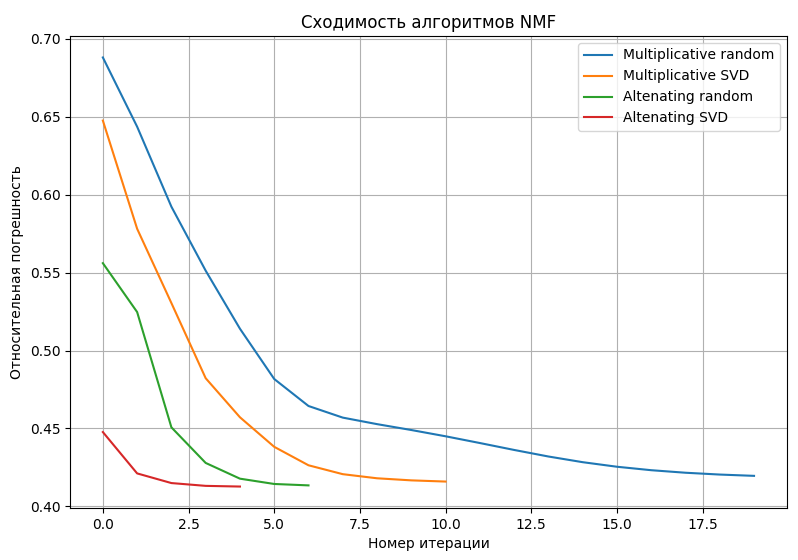
\includegraphics[width=\linewidth]{assets/Graph1.png}
  \caption{График относительной погрешности}
  \label{fig:relativeApproximationError}
\end{figure}

\newpage


Ниже приведены данные показывающие затраты по времени на выполнение алгоритмов:
\\

\begin{lstlisting}[caption=Затраты по времени на выполнение алгоритмов]
# Initialization:
Random takes 2.002e-05s
SVD takes 4.435e-04s
# Methods:
Multiplicative random takes 3.202e-03s
Multiplicative SVD takes 6.939e-04s
Altenating random takes 1.151e-02s
Altenating SVD takes 6.742e-03s
\end{lstlisting}

Ниже приведены результаты алгоритма попеременных наименьших квадратов с использованием SVD инициализации:

\begin{align*}
W H =
\begin{pmatrix}
     0.153  &   0  &   0.089 \\
     0  &   0  &   0.518 \\
     0  &   0  &   0.518 \\
     0.372  &   0.099  &   0 \\
     0.237  &   0  &   0 \\
     0  &   0.516  &   0 \\
     0.525  &  	0  &   0.027 \\
     0.042  &   0.752  &   0 \\
     0.229  &   0.131  &   0.613 \\
     0.042  &   0.752  &   0
\end{pmatrix}
\begin{pmatrix}
     2.152  &   0  &   1.897  &   1.530  &  0 \\
     0  &   1.472  &   1.022  &   0  &   0 \\
     0  &   0  &   0.250  &   0.493  &   1.844
\end{pmatrix}
\end{align*}



\newpage



Полученные данные можно интерпретировать в виде следующих таблиц:

\begin{center}
 \begin{tabular}{ l | c c c c c c }
 Термин      & 1 & 2 & 3 \\
 \hline
 eigenvalue  & 0.153  &   0  &   0.089 \\
 England     & 0  &   0  &   0.518 \\
 FIFA        & 0  &   0  &   0.518 \\
 Google      & 0.372  &   0.099  &   0 \\
 Internet    & 0.237  &   0  &   0 \\
 link        & 0  &   0.516  &   0 \\
 matrix      & 0.525  &  	0  &   0.027 \\
 page        & 0.042  &   0.752  &   0 \\
 rank        & 0.229  &   0.131  &   0.613 \\
 Web         & 0.042  &   0.752  &   0
\end{tabular}
\end{center}

\begin{center}
 \begin{tabular}{ l | c c c c c c }
 Вектор      & Док 1 & Док 2 & Док 3 & Док 4 & Док 5 \\
 \hline
 1           & 2.152  &   0  &   1.897  &   1.530  &  0 \\
 2           & 0  &   1.472  &   1.022  &   0  &   0 \\
 3           & 0  &   0  &   0.250  &   0.493  &   1.844 \\
\end{tabular}
\end{center}

\newpage

\subsection{Вывод}

На Рис.~\ref{fig:relativeApproximationError} отчётливо видно,
что мультипликативным алогритмам необходимо в 2-3 раза больше итераций, чтобы добиться заданной точности.
Также график показывает, что мультипликативные алгоритмы чаще сходятся к более \say{плохой} точке локального минимума,
которая даёт меньшую точность разложения.
Касательно алгоритмов попеременных наименьших квадратов видно, что даже после первой итерации
относительная ошибка значительно меньше чем у предыдущих алгоритмов и в целом они требуют намного меньше итераций.

В обоих случаях инициализация матриц $W$ и $H$ с помощью сингулярного разложения понижает ошибку на первой итерации и уменьшает количество итерации.

Напомним, что первые четыре документа рассказывают о Google и рейтинге веб-страниц,
а пятый касается футбола. Из таблиц можно увидеть, что первые четыре документа представлены векторами,
которые имеют большие компоненты для ключевых слов, связанных с Google.
В отличие от этого, пятый документ представлен только третьим базисным вектором, так же с большой компонентой.
Мы видим, что третий вектор представляет документы рассказывающие о футболе, а два других показывают документы, связанные с Google.






\newpage





\section{Вычислительные эксперименты на разреженных данных}

\subsection{Эксперимент 1}

Для тестирования алгоритмов на больших разреженных данных
было построено разложение ранга $k = 25$ с использованием терм-документной матрицы размера $6947 \times 3837$,
построенной на основе романа \say{Пикник на обочине}.
В критерии остановки итераций \eqref{eq:termination} $\epsilon = 10^{-3}$.

\begin{tikzpicture}[
  trim axis left,
  every mark/.append style={mark size=4pt},
]
  \begin{axis}[
    axis lines = left,
    scale only axis,
    grid = major,
    title = График сходимости алгоритмов,
    xlabel = Номер итерации,
    ylabel = Ошибка,
    width = 0.9\textwidth,
    height = 0.7\textwidth,
    enlarge x limits={0.05},
    enlarge y limits={0.05},
    line width=1pt,
  ]

    \addplot table [
      x=iteration,
      y=roadside_picnic.25.ALS_LSQR,
      col sep=comma,
      skip coords between index={0}{1},
    ] {../samples/data.csv};
    \addlegendentry{ALS\_LSQR - 639s}

    \addplot table [
      x=iteration,
      y=roadside_picnic.25.ALS_NNLS,
      col sep=comma,
      skip coords between index={0}{1},
    ] {../samples/data.csv};
    \addlegendentry{ALS\_NNLS - 412s}

    \addplot table [
      x=iteration,
      y=roadside_picnic.25.ALS_NORM,
      col sep=comma,
      skip coords between index={0}{1},
    ] {../samples/data.csv};
    \addlegendentry{ALS\_NORM - 0.5s}

    \addplot table [
      x=iteration,
      y=roadside_picnic.25.MU,
      col sep=comma,
      skip coords between index={0}{1},
    ] {../samples/data.csv};
    \addlegendentry{MU - 0.7s}

  \end{axis}
\end{tikzpicture}

\begin{itemize}
  \item ALS\_LSQR - Метод попеременных наименьших квадратов на основе алогитма LSQR
  \item ALS\_NNLS - Метод попеременных неотрицательных наименьших квадратов
  \item ALS\_NORM - Метод попеременных наименьших квадратов на основе нормальных уравнений
  \item MU - Метод мультипликативного обновления
\end{itemize}

В виду резкого снижения погрешности после первой итерации, на графиках сходимости не указана погрешность нулевого приближения.
В рассматриваемом случае погрешность равна $1024008.859$.

\begin{figure}[h]
  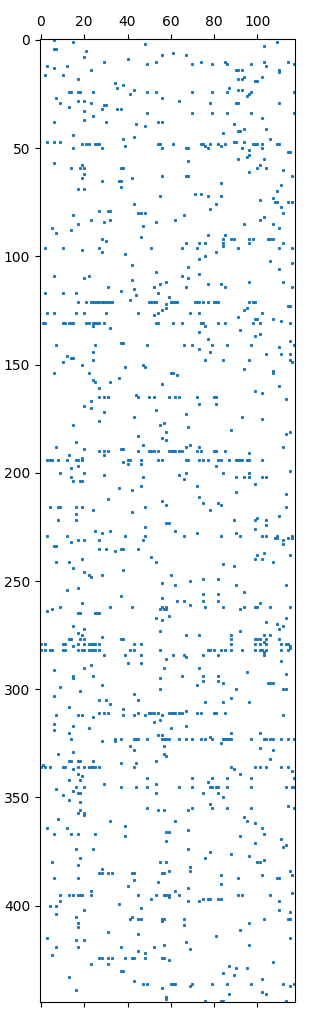
\includegraphics[width=0.3\linewidth]{assets/SparsityPattern.png}
  \caption{Структура разреженности терм-документной матрицы, построенной на основе романа "Пикник на обочине"}
  \label{fig:SparsityPattern}
\end{figure}
\newpage


\subsection{Эксперимент 2}

Следующий график показывает зависимость ошибки получаемого разложения в зависимости от ранга разложения.
Для проведения данного опыта в качестве основы был взят текст первой главы настоящей работы.
Полученная терм-документная матрица состоит из 445 столбцов и 118 строк.
В критерии остановки итераций \eqref{eq:termination} $\epsilon = 10^{-3}$.
Эксперимент проводится с использованием метода попеременных наименьших квадратов на основе нормальных уравнений (ALS\_NORM).

\begin{tikzpicture}[
  trim axis left,
  every mark/.append style={mark size=1pt},
]
  \begin{axis}[
    axis lines = left,
    scale only axis,
    grid = major,
    title = График зависимости ошибки от ранга,
    xlabel = Ранг,
    ylabel = Ошибка,
    width = 0.9\textwidth,
    height = 0.7\textwidth,
    enlarge x limits={0.05},
    enlarge y limits={0.05},
    line width=1pt,
  ]

    \addplot table [
      x=rank,
      y=error,
      col sep=comma,
    ] {../samples/rank-error.csv};

  \end{axis}
\end{tikzpicture}

\newpage

\subsection{Выводы}

Эксперимент 1 показывает, что метод попеременных неотрицательных наименьших квадратов (ALS\_NNLS)
сходится к самому \say{лучшему} приближению, так как каждый шаг неотрицательных наименьших квадратов
не требует дополнительного проецирования результата на неотрицательную область.
Однако метод требует большое количество вычислительных ресурсов, так как шаги неотрицательных наименьших квадратов
не приспособлены к работе с большими разреженными матрицами.

Самым эффективным методом среди рассмотренных является метод попеременных наименьших квадратов на основе нормальных уравнений,
так как данный метод даёт \say{достаточно хорошее} приближения за наименьшее время.

Эксперимент 2 показывает, что при увеличении ранга $k$ аппроксимации методы начинают сходиться к более \say{глубоким} локальным минимумам.
Это можно объяснить тем, что при аппроксимации малым рангом происходит некоторое \say{сжатие} данных или выделение \say{важных} данных, и чем больше ранг аппроксимации,
тем легче методам сойтись к более \say{глубокому} локальному минимуму.

\newpage





\section{Вычислительный эксперимент на задачах интеллектуального анализа текста}

Для проведения данного опыта в качестве основы взят текст первой главы настоящей работы.
Для каждой рассмотренной задачи проведено выделение 5 ключевых предложений.
Анализ результата проведём в следующей секции.


\subsection{Результат метода оценки значимости}

\begin{itemize}
  \item Ключевой характеристикой неотрицательной матричной факторизации является возможность
  использования численных методов для минимизации \eqref{eq:min_problem}
  для извлечения некоторых базовых признаков в качестве базисных векторов матрицы $W​$,
  которые затем могут быть использованы для поиска и классификации.
  \item Несмотря на многие недостатки неотрицательная матричная факторизация весьма привлекательна для приложений интеллектуального анализа данных,
  поскольку на практике даже локальные минимумы могут обеспечивать желаемые свойства, такие как сжатие данных и извлечение базовых признаков.
  \item Эта блокировка нулевых элементов является большим ограничением алгоритма,
  что означает как только алгоритм начинает двигаться вниз по пути к фиксированной точке,
  даже если это \say{плохая} фиксированная точка, алгоритм продолжит двигаться в направлении к этой точке.
  \item Численные методы решения задачи неотрицательной матричной факторизации могут быть поделены на следующие основные категории: 	Методы мультипликативного обновления, 	Методы попеременных наименьших квадратов, 	Методы градиентного спуска.
  \item Стоит отметить что все вышеперечисленные методы решают задачу неотрицательной матричной факторизации,
однако название \textit{"метод неотрицательной матричной факторизации"} обычно применимо только к методам решающим задачу в формулировке \eqref{eq:min_problem}.
\end{itemize}


\newpage


\subsection{Результат метода извлечение ключевых предложений из аппроксимации ранга $k = 5$}

\begin{itemize}
  \item Эта блокировка нулевых элементов является большим ограничением алгоритма,
  что означает как только алгоритм начинает двигаться вниз по пути к фиксированной точке,
  даже если это \say{плохая} фиксированная точка, алгоритм продолжит двигаться в направлении к этой точке.
  \item Ниже будет использован несколько модифицированный вариант нормы Фробениуса, который будем называть относительной погрешностью нормы Фробениуса.
  \item  Ключевой характеристикой неотрицательной матричной факторизации является возможность
  использования численных методов для минимизации \eqref{eq:min_problem}
  для извлечения некоторых базовых признаков в качестве базисных векторов матрицы $W​$,
  которые затем могут быть использованы для поиска и классификации.
  \item Несмотря на многие недостатки неотрицательная матричная факторизация весьма привлекательна для приложений интеллектуального анализа данных,
  поскольку на практике даже локальные минимумы могут обеспечивать желаемые свойства, такие как сжатие данных и извлечение базовых признаков.
  \item Численные методы решения задачи неотрицательной матричной факторизации могут быть поделены на следующие основные категории: 	Методы мультипликативного обновления, 	Методы попеременных наименьших квадратов, 	Методы градиентного спуска.

\end{itemize}

\newpage

\subsection{Выводы}

Метод, основанный на оценках значимости, имеет недостаток:
если в тексте присутствуют два и более \say{самых значимых предложения}, которые содержат одинаковые термы высокой значимости,
то их координаты будут примерно одинаковыми, и оба предложения будут извлечены как ключевые.
Но это не практично со стороны поиска информации, так как они очень похожи.

По результатам видно, что оба метода предпочитают более длинные предложения.

Также по результатам можно понять, что метод извлечение ключевых предложений из
аппроксимации ранга $k$ старается включить в выборку предложения касающиеся \say{ортогональных} тем.
Под \say{ортогональностью} тем подразумевается их разнородность и в некоторой мере субъективная оценка.
Такие свойства метода напрямую вытекают из использования $QR$ разложения.

Учитывая всё вышесказанное, можно сделать вывод, что метод извлечение ключевых предложений из
аппроксимации ранга $k$ даёт более качественную выборку, однако требует больше вычислительных ресурсов.

	% Заключение (еще раз повторить постановку, четко обозначить то, что было сделано и основные полученные результаты исследования)

\chapter*{Заключение}
\addcontentsline{toc}{chapter}{Заключение}

В ходе работы была рассмотрена и исследована задача неотрицательной матричной факторизации, которая формулируется следующим образом.

Для матрицы $A \in R^{m \times n}, A \geq 0$ и числа $k \in N, k < \min\{n, m\}$
необходимо найти матрицы $W \in R^{m \times k}, H \in R^{k \times n} : W \geq 0, H \geq 0$ минимизируя функционал:
\begin{equation*}
  \min_{W \leq 0, \ H \leq 0} \dfrac{||A - WH||_F}{|| A ||_F}
\end{equation*}

Также были рассмотрены и реализованы эффективные алоритмы решения этой задачи.

Алгоритмы были успешно применены на практике для решения проблем интеллектуального анализа текста.

Таким образом, рассмотренные алгоритмы неотрицательной матричной факторизции
эффективны и надежны для извлечения и разделения статистически зависимых данных.
Тем не менее, проблема, которая все еще остается нерешённой, состоит в том,
чтобы доказать глобальную сходимость таких алгоритмов и оценить скорости сходимости данных алгоритмов.


	\begin{thebibliography}{9}
		\bibitem{berry} Michael W. Berry, Murray Browne, Amy N. Langville, V. Paul Pauca, Robert J. Plemmons, Algorithms and applications for approximate nonnegative matrix factorization, Computational Statistics; Data Analysis, Volume 52, Issue 1, 2007, p. 155-173.
		\bibitem{elden} Lars Eldén. 2007. Matrix Methods in Data Mining and Pattern Recognition (Fundamentals of Algorithms). Soc. for Industrial and Applied Math., Philadelphia, PA, USA.
		\bibitem{demmel} Деммель Дж. Вычислительная линейная алгебра. М.: Мир, 2001.
		\bibitem{habr} Интернет ресурс 'Habr'. https://habr.com/ru/post/264375/
	\end{thebibliography}

\end{document}
